\section{Previous work in Cardinal}
\label{s:cardinal}

MOOSE was originally developed for solving fully coupled systems of partial differential equations (PDEs)
using fully implicit timestepping. To utilize MOOSE developers create small C++ objects which represent
their partial differential equations, boundary conditions, initial conditions, etc. MOOSE will then coordinate PETSc and libMesh to perform a Newton solve over all of the physics to find the solution to the multiphysics problem. While this is still the primary way to use MOOSE, the library has also gained capability for loosely coupled solves, Picard iteration and even coupling to external applications (such as OpenMC and Nek5000).
Disussion on the MultiApp features of MOOSE used in Cardinal are provided in [].

When utilizing MOOSE to couple multiple disparate codes together a new MOOSE-based application was created [] which compiles all of the codes into one executable. For the previous study that code was  named Cardinal and combines BISON, OpenMC and Nek5000 to achieve high-fidelity simulation of FHR reactors.

\subsection{Design of Cardinal}
\label{ss:c1}

Cardinal utilizes the MOOSE MultiApp capability to place each of the applications to be coupled within
a hierarchical tree-based structure as shown in \ref{f:cardinal}. This structure was chosen based on how tightly
coupled the physics are. BISON and Nek5000 form one branch due to the instantaneous feedback between the conjugate heat transfer and the pebble temperature. The Nek5000 solution provides the temperature boundary condition on the exterior of each pebble while BISON returns the heat  flux at each point around
the pebble to Nek5000. Another benefit of having BISON and Nek5000 on their own branch is the way it impacts timestepping. Within the MultiApp setup shown in Figure \ref{f:cardinal} the branch containing BISON and Nek5000 can take many small timesteps, and even iterate between BISON and Nek5000 within a timestep, without needing to re-solve OpenMC. This greatly increases the runtime speed of the application.OpenMC is then separate from the other two. It receives fuel/pebble temperatures from BISON and returns a heat source which is transferred down to BISON. OpenMC is currently solving for steady state neutronics and can therefore take larger timesteps compared to BISON and Nek5000 (which are both performing transient heat conduction and CFD solves respectively). The flexibility of the MOOSE MultiApp system allows for just such a setup. Discussions on the related APIs for each of the codes mentioned are contained in the previous report \cite{cardinal}.

\begin{figure}[!h]
\centering
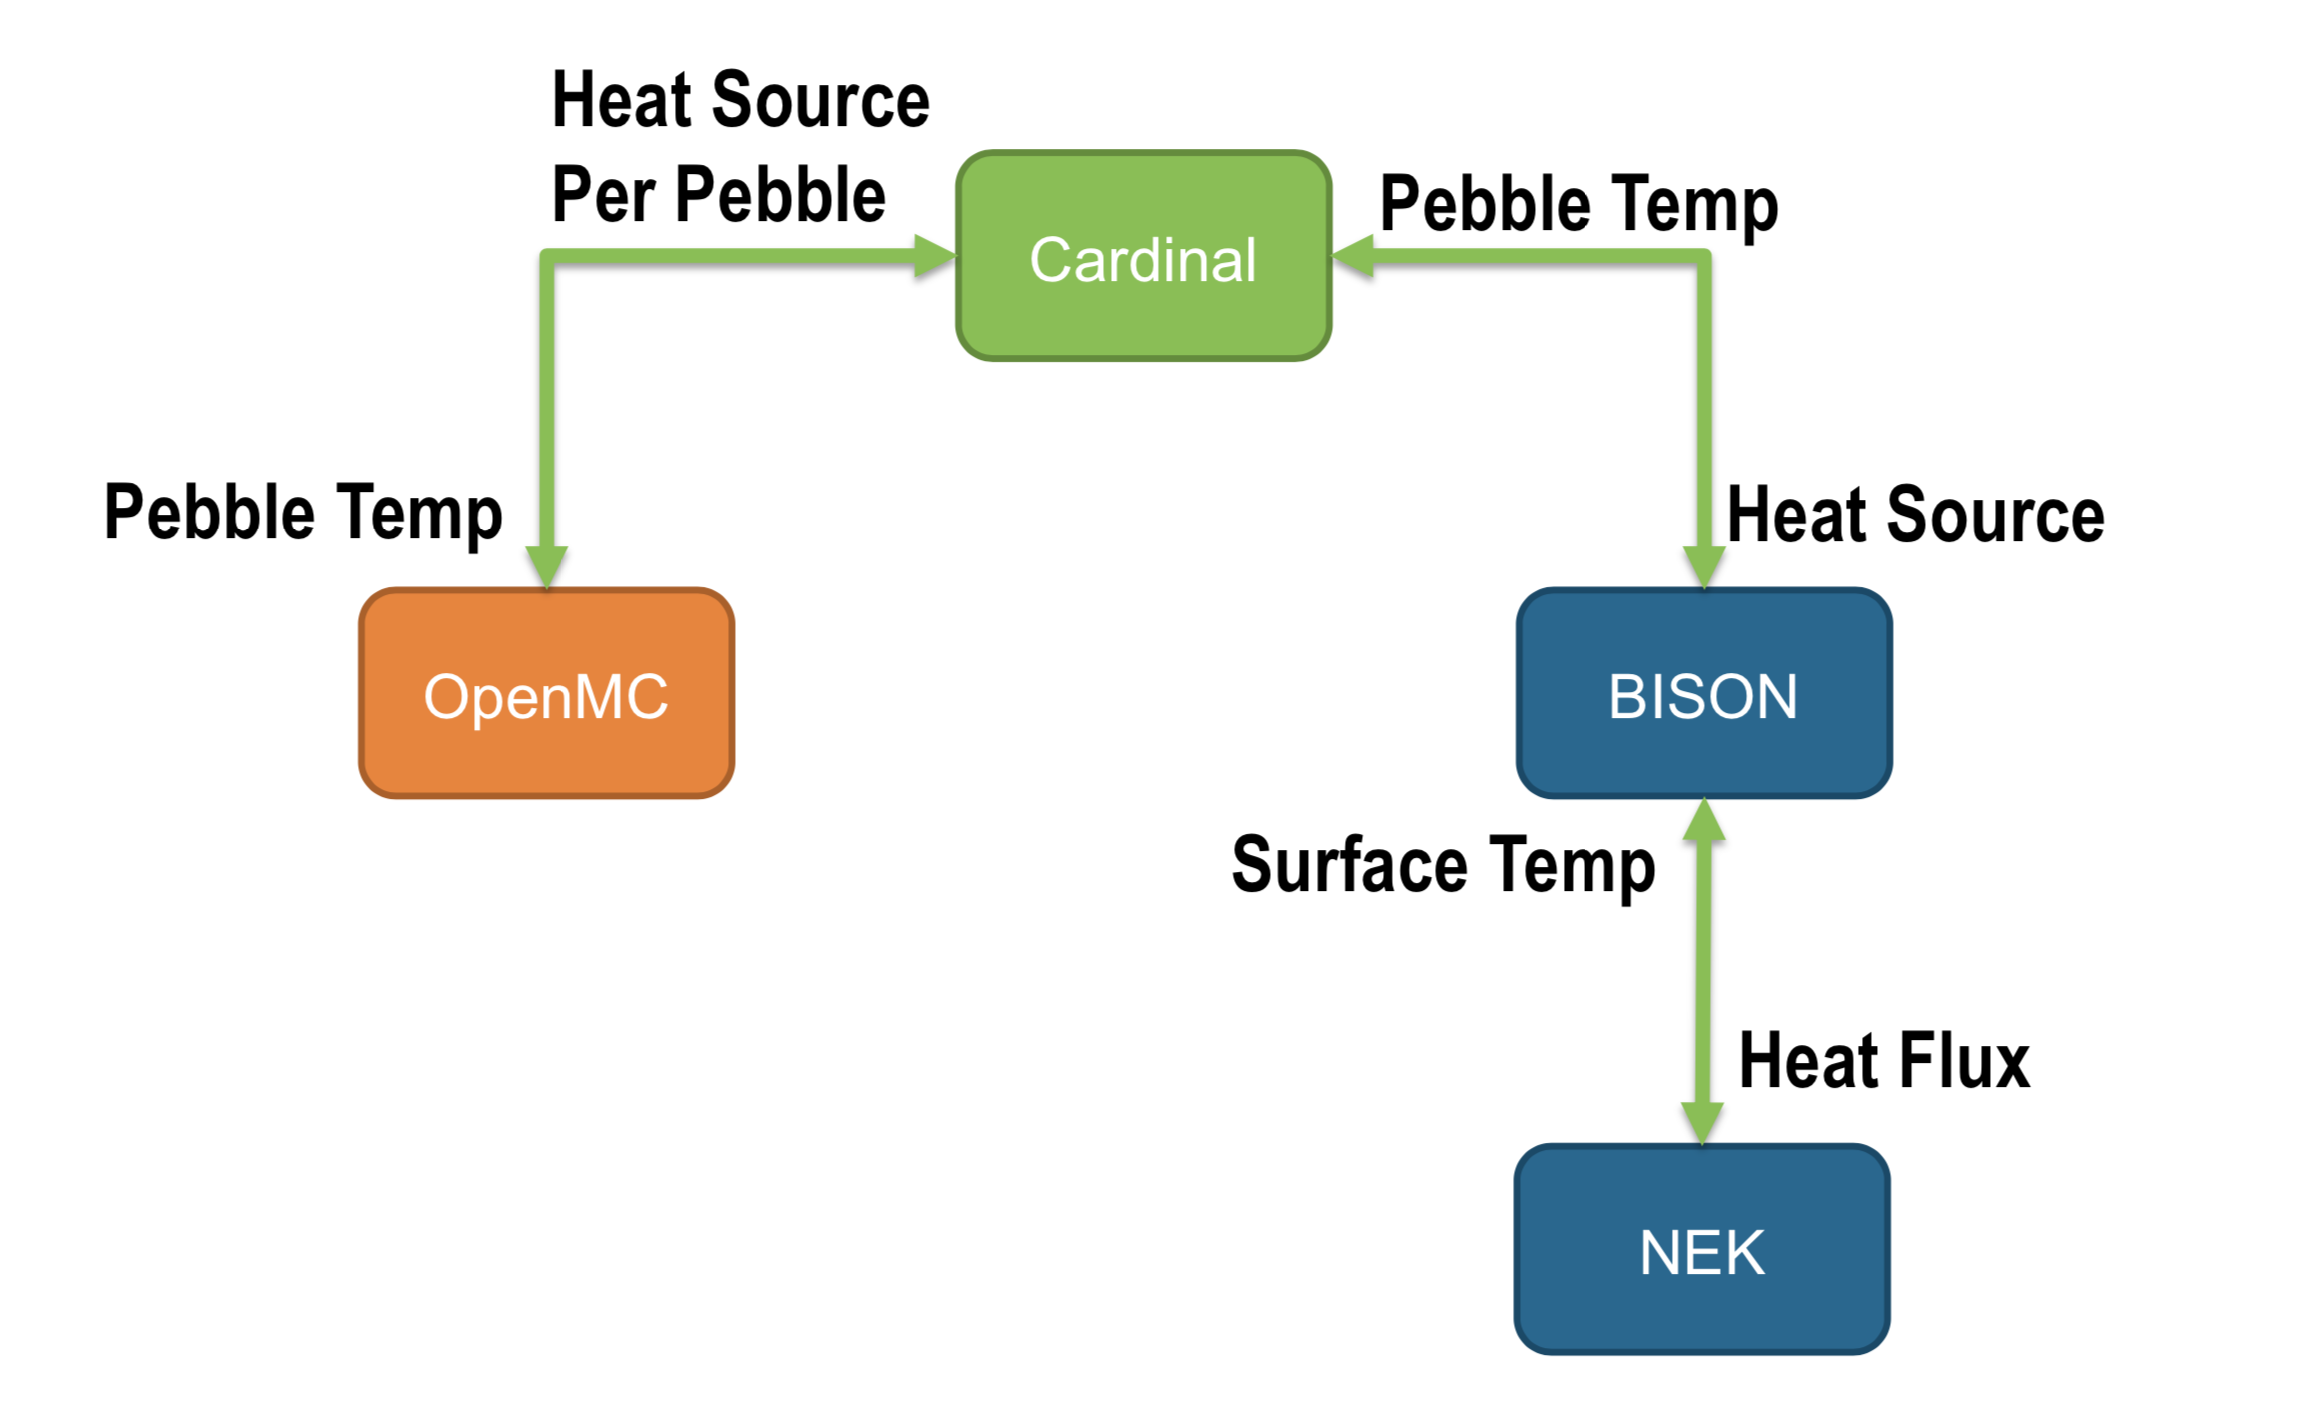
\includegraphics[clip=true,width=0.9\textwidth]{Figures/cardinal}
\caption{Diagram showing the design of Cardinal.}
\label{f:cardinal}
\end{figure}

This structure has been updated in the present report to allow for NekRS to be used instead of Nek5000 allowing for execution of the fluid problem (by far the most expensive of the three) on GPUs.

\subsection{Build system}
\label{ss:c2}

All libraries get config info from PETSc for consistent compilation. After installing PETSc and libmesh, Cardinal can be built in one step.

\begin{figure}[!h]
\centering
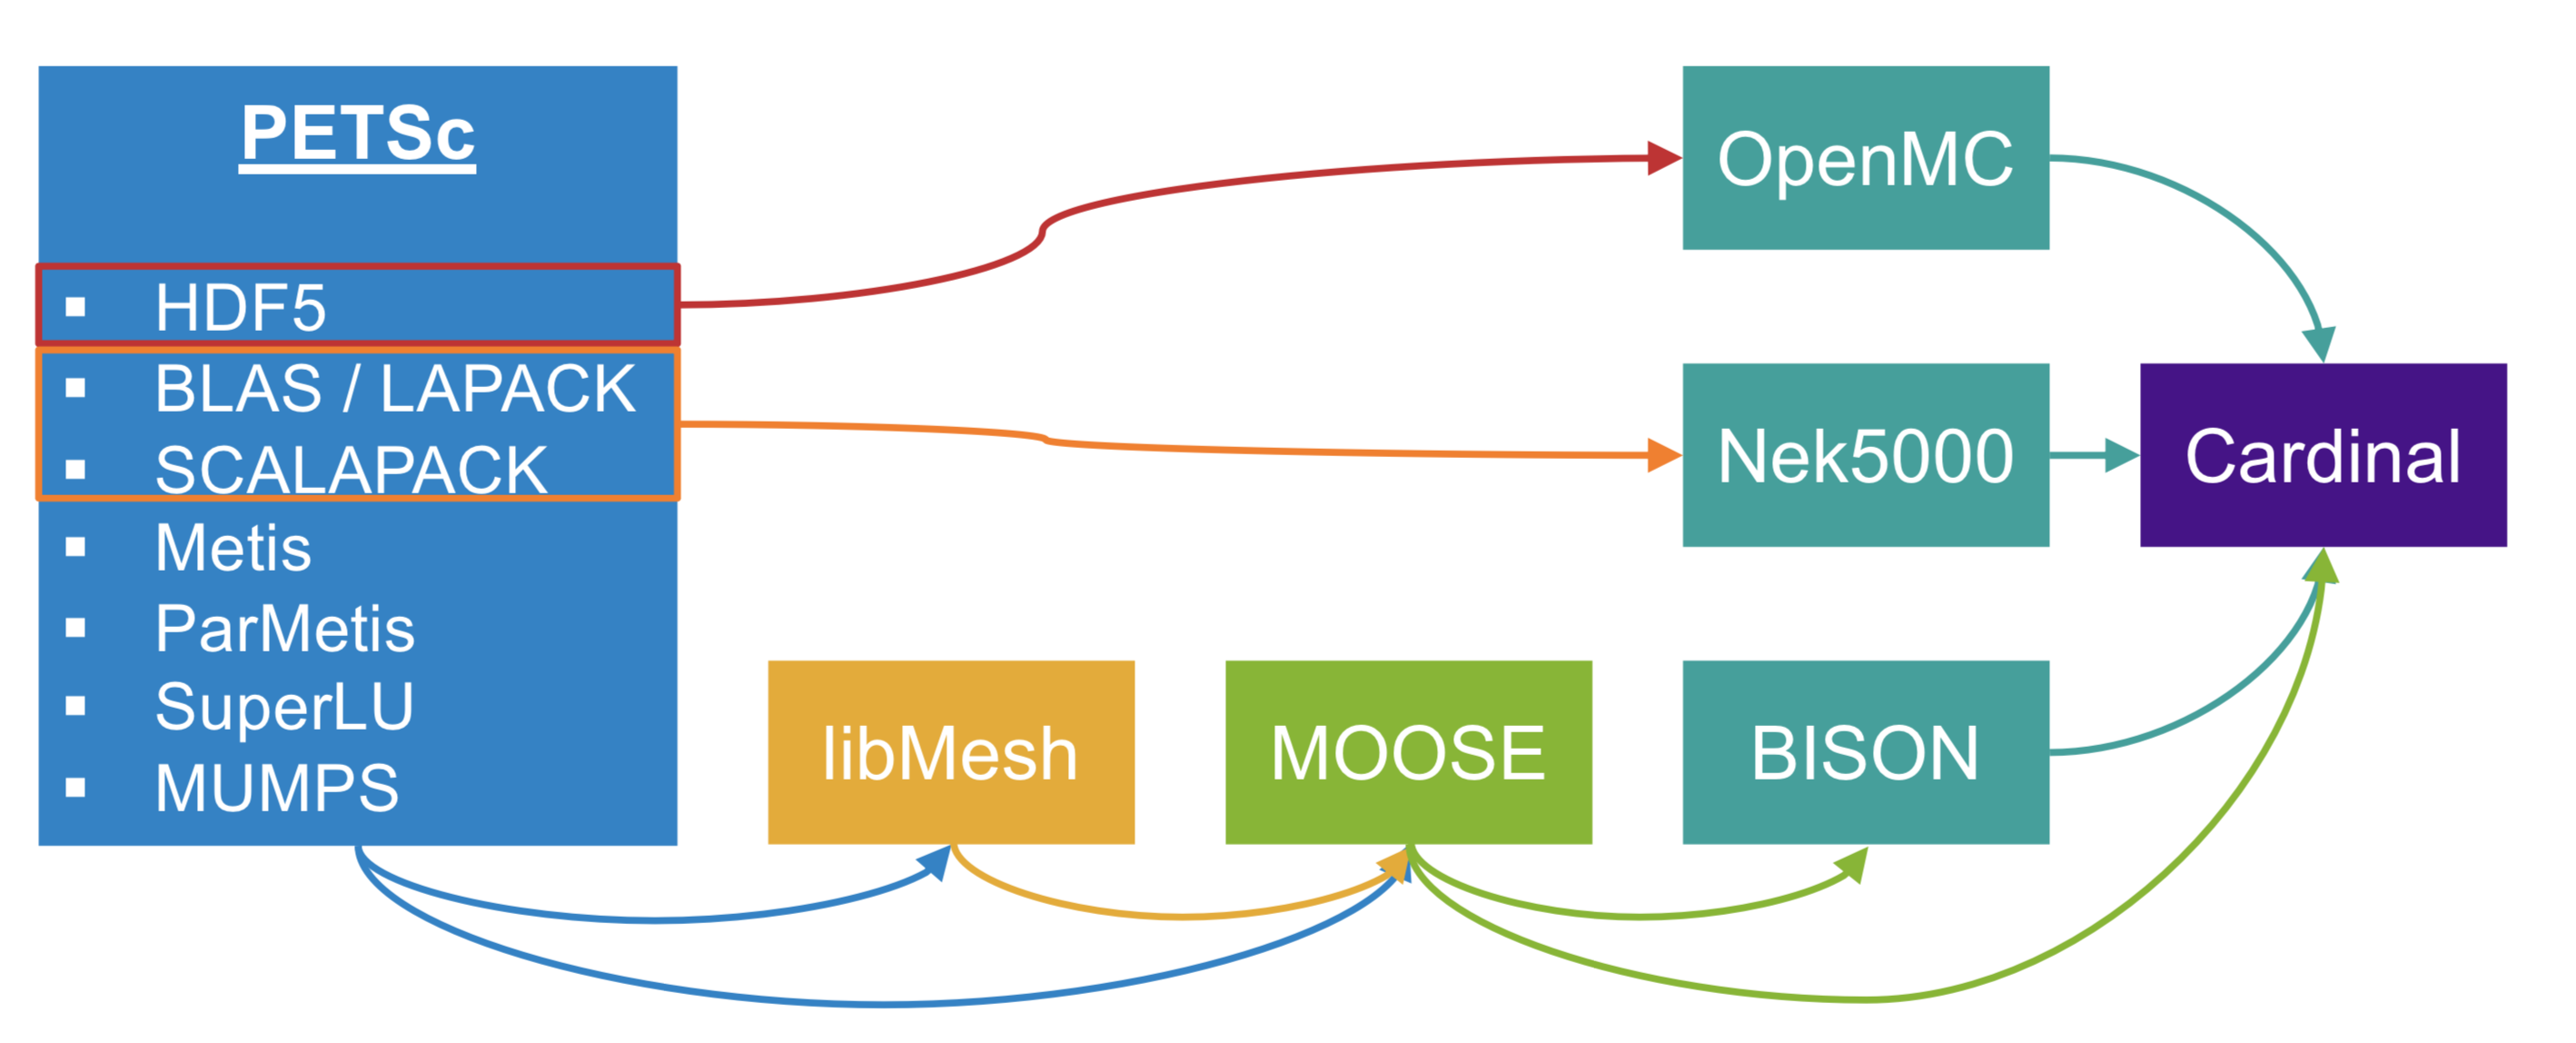
\includegraphics[clip=true,width=0.9\textwidth]{Figures/build}
\caption{Diagram describing the build system of Cardinal.}
\label{f:build}
\end{figure}

The build system of Cardinal has largely been kept intact for the present work. We have however added a branch of the repository that compiles NekRS instead of Nek5000. The build system has also been updated to allow Cardinal to run on the ORNL supercomputer Summit.

\subsection{Verification and validation}
\label{ss:c3}

In order to verify the fluid flow model and the solution transfer we have devised two cases including a single pebble and a two pebble case. The Nek5000-MOOSE coupling was verified to yield the same results as
stand-alone Nek5000 conjugate heat transfer results. We note that work in Cardinal was based on previous
work conducted on Nek5000-MOOSE coupling \cite{novak2018preliminary}. The single pebble Figure~\ref{f:pb1} and two pebble (Figure~\ref{f:pb2}) were also used to verify the OpenMC and BISON coupling. For instance the neutronics results showed a clear bias between pebbles and a tilt induced by the temperature gradient.

\begin{figure}[!h]
\centering
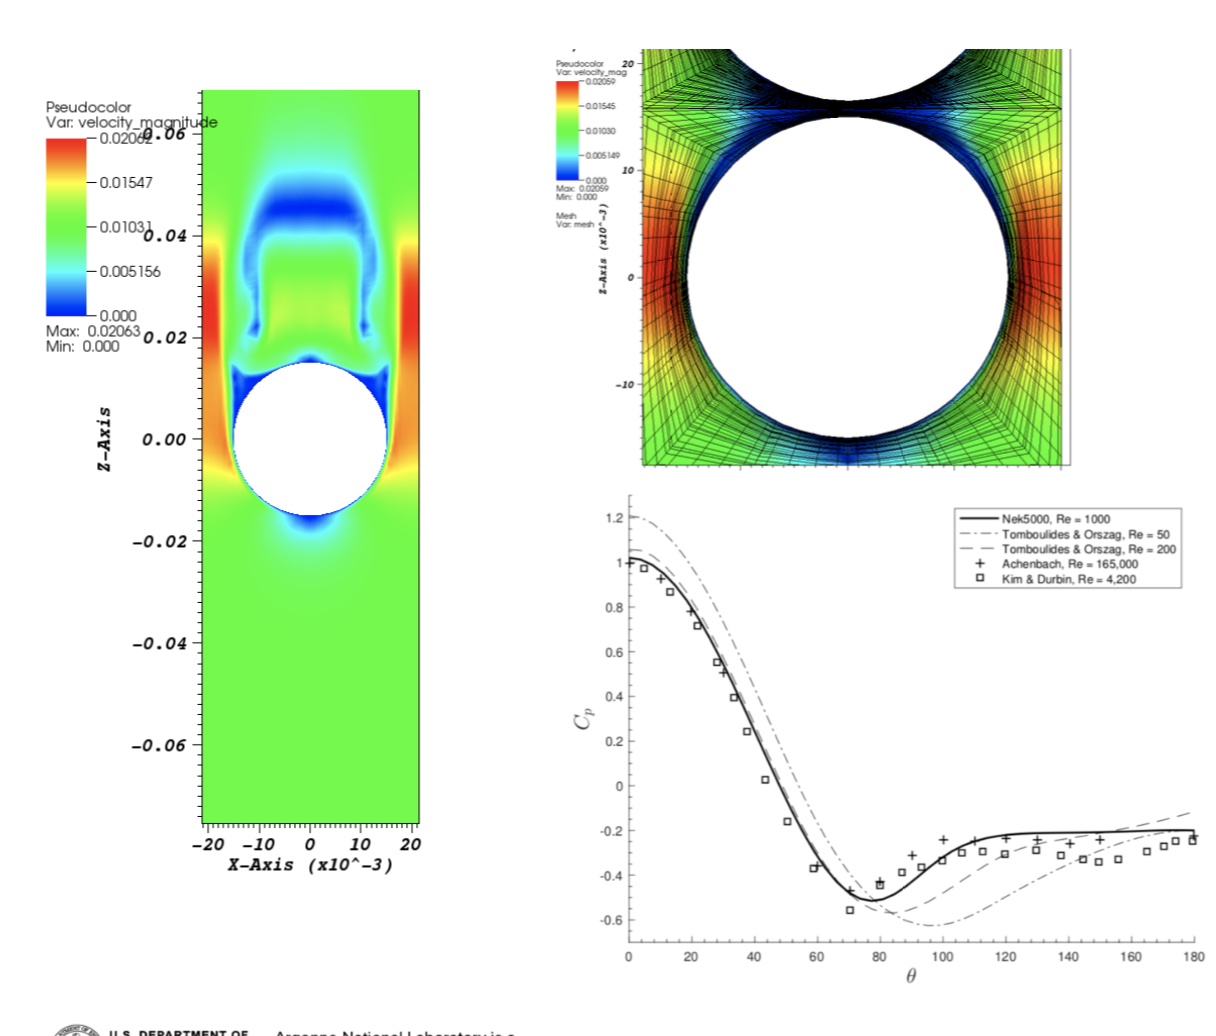
\includegraphics[clip=true,width=0.9\textwidth]{Figures/pb_vv1}
\caption{Verification test - Single pebble and comparison with experiment.}
\label{f:pb1}
\end{figure}

\begin{figure}[!h]
\centering
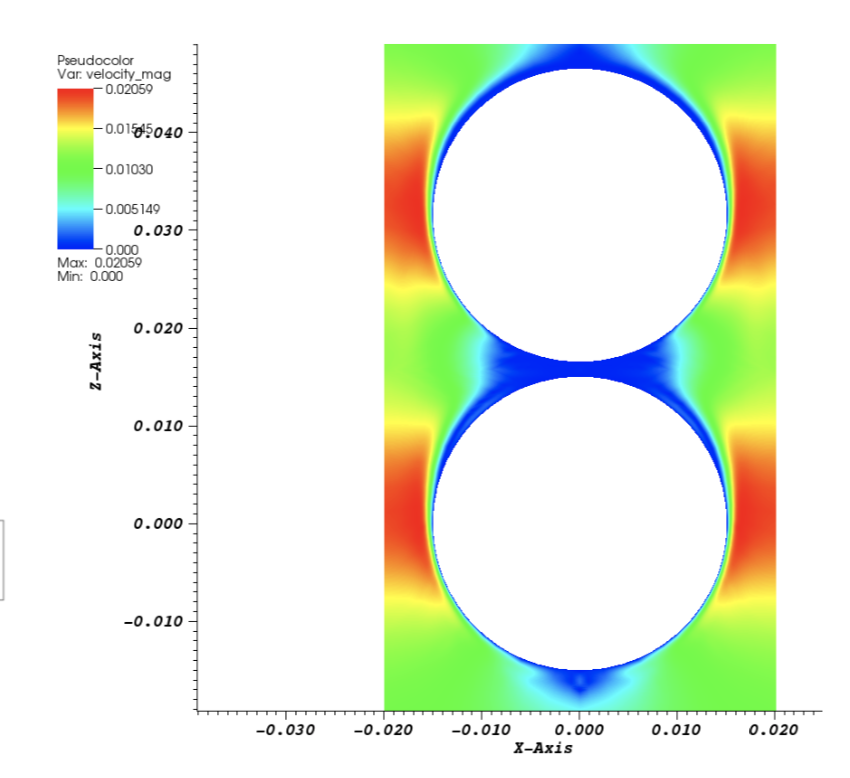
\includegraphics[clip=true,width=0.6\textwidth]{Figures/pb_vv2}
\caption{Verification test - Two pebbles.}
\label{f:pb2}
\end{figure}

Selected results from the single pebble case were also ompared with results from experimental and computational studies carried out by using a similar geometries \ref{fig:pb1}. A well quantified quantity for flow over a single-sphere is the averaged stream- wise velocity along the domain axial center line. Figure~\ref{fig:pb2} compares our result with completed numerical results. The figure shows the profile generated from DNS data in \cite{fick2017investigation} at $Re = 3,700$ and shows the downstream location ($z=D$) and magnitude of the maximum recirculation (i.e. negative streamwise) velocity for LES and DES data generated at Re = 10; 000. One can see that for increasing Reynolds number, the magnitude of the recirculation velocity increases, while the downstream distance from the sphere where this maximum occurs, decreases. We do not quantify the specific dependence of this trend on the Reynolds number here, but our result to be consistent with the literature.
Over the past several years NEAMS has dedicated several efforts to the modeling and simulation of the detailed flow in a pebble bed. For instance, Fick et al. \cite{fick2017direct}  performed a complete Direct Numerical Simulation of pebble bed flow. Complete statistical data was obtained from this DNS study, with an investigation of low-frequency temporal instabilities. However, Ficks study \cite{fick2017direct} used a structured pebble bed, which limits its application. Nonetheless it was compared against other available DNS data and proved Nek5000 can deliver high quality simulation data for pebble beds. A more recent study aimed at simulating the flow in a random pebble bed \cite{yildiz2020direct}. This random pebble bed geometry was obtained from an experiment conducted by Nguyen et .al \cite{nguyen2018time}. However, only a small section of the whole domain from the experiment was studied. A picture of the experimental facility is shown in Figure~\ref{f:tamu1}, while a snapshot of the PIVfield examined is shown in Figure~\ref{f:tamu2}.

To create pure hexahedral mesh for random pebble bed is very challenge if using tradition blocking method. However, with tet-to-hex meshing method, we could create pure hexahedral mesh for this geometry. To reduce total elements number, chamfers are created at pebble-pebble interaction. As we discussed, the computational domain is only a small section of the whole experimental domain, therefore we applied periodic boundary condition at inlet/outlet to mimic the upstream/downstream. Figure~\ref{f:tamu3} shows the instantaneous velocityeld at cross sections of the random pebble bed, as well as the near wall mesh at pebble surface. In Figure~\ref{f:tamu4}, the flow field is very complex due to randomly distributed pebble. Despite the complexity of the geometry  the computational results compared favorably.

\begin{figure}[!h]
\centering
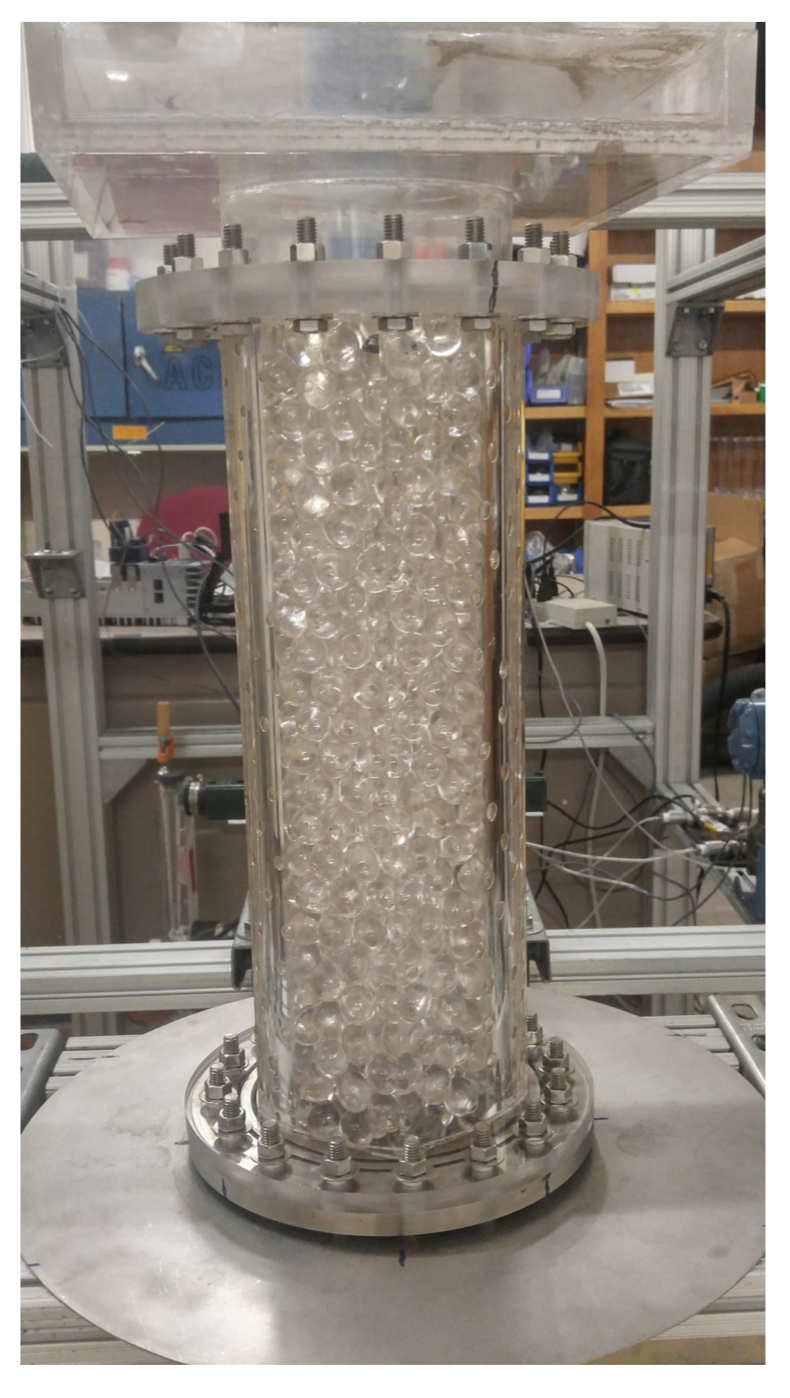
\includegraphics[clip=true,width=0.5\textwidth]{Figures/pb_tamu1}
\caption{TAMU experiment - Picture of the facility. }
\label{f:tamu1}
\end{figure}

\begin{figure}[!h]
\centering
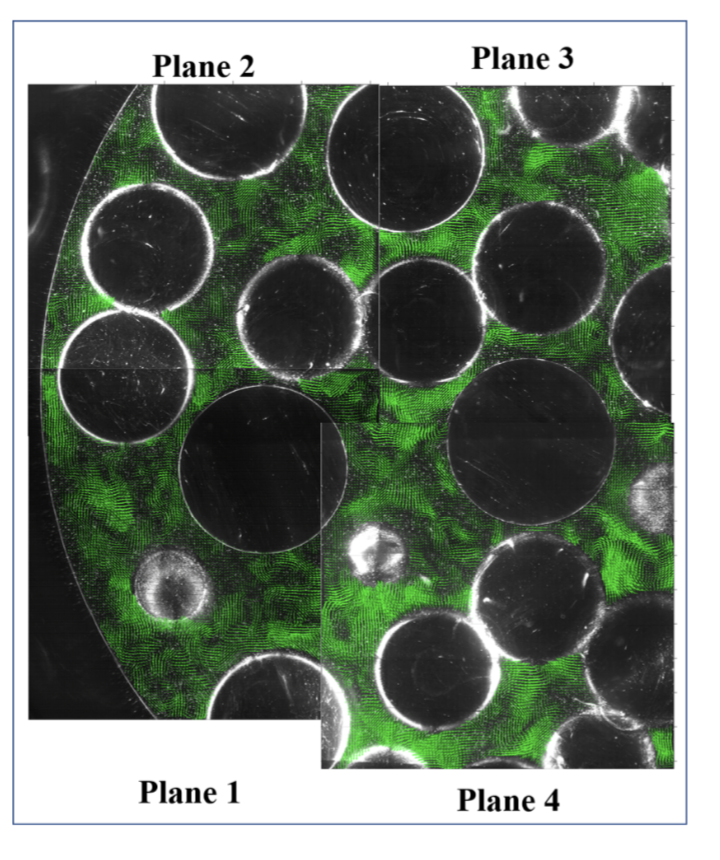
\includegraphics[clip=true,width=0.5\textwidth]{Figures/pb_tamu2}
\caption{TAMU experiment - PIV snapshot.}
\label{f:tamu2}
\end{figure}

\begin{figure}[!h]
\centering
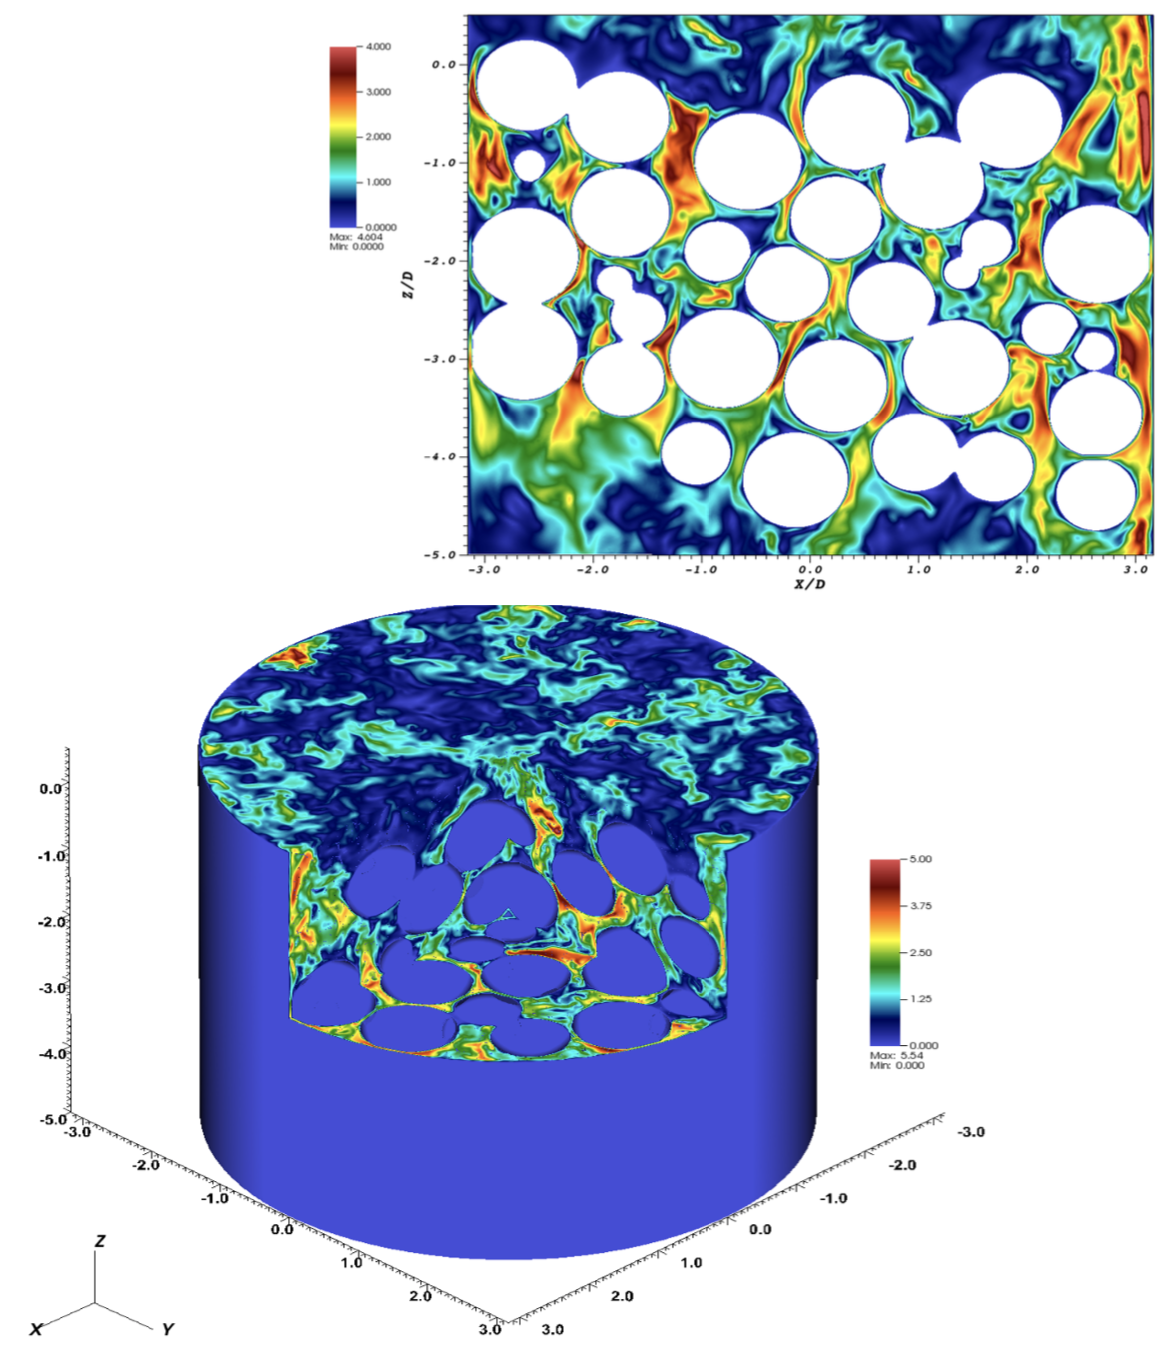
\includegraphics[clip=true,width=0.9\textwidth]{Figures/pb_tamu3}
\caption{TAMU experiment - Simulation results.}
\label{f:tamu3}
\end{figure}

\begin{figure}[!h]
\centering
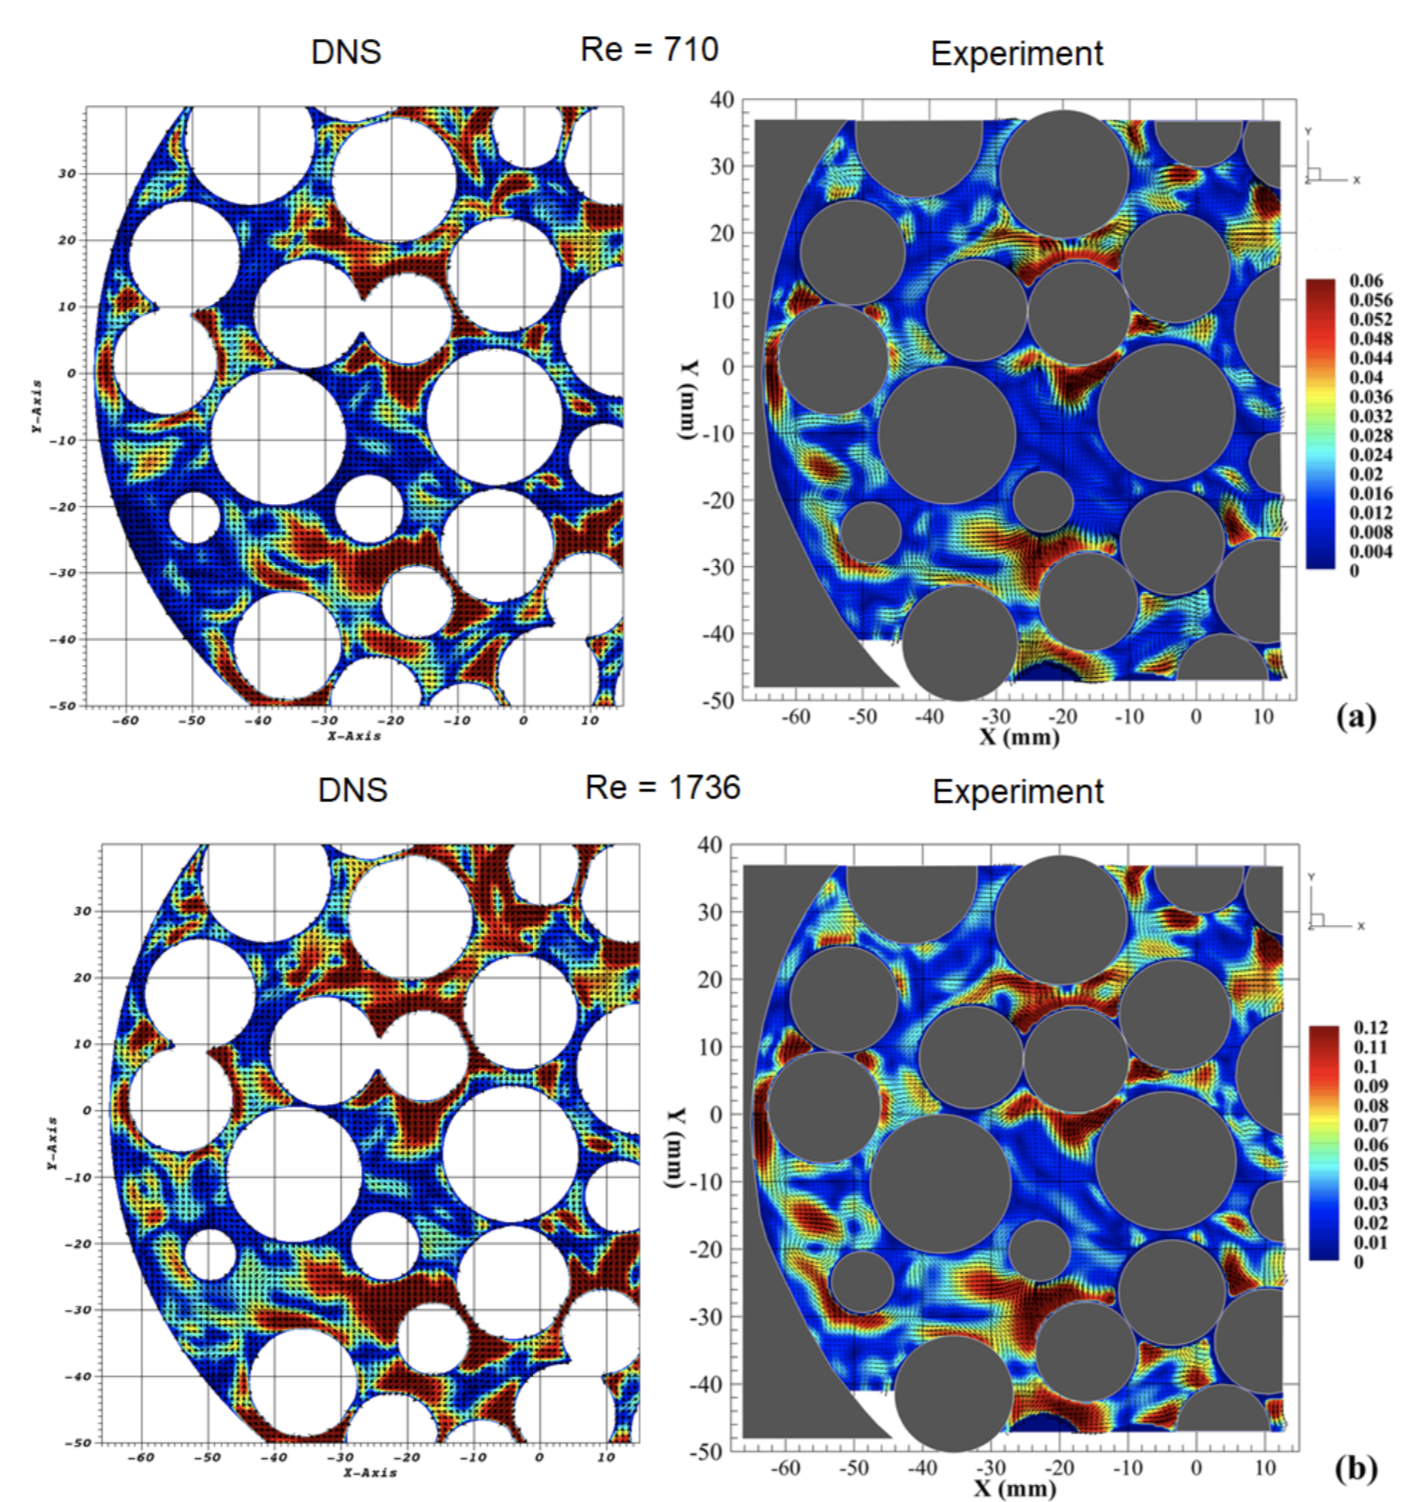
\includegraphics[clip=true,width=0.9\textwidth]{Figures/pb_tamu4}
\caption{TAMU experiment - Comparison with experiment. }
\label{f:tamu4}
\end{figure}

\subsection{Previous coupled simulations}
\label{ss:c4}

Using as a basis the Nek5000 model of TAMU experiment, we have developed a multi-physics simulation of a bed comprising 146 pebbles. The numerical setup and results are discussed in more detail in \cite{cardinal}. We report here only some select results on the average temperature distribution and power distribution (Figure~\ref{f:dtamu1} and Figure~\ref{f:dtamu2}).

\begin{figure}[!h]
\centering
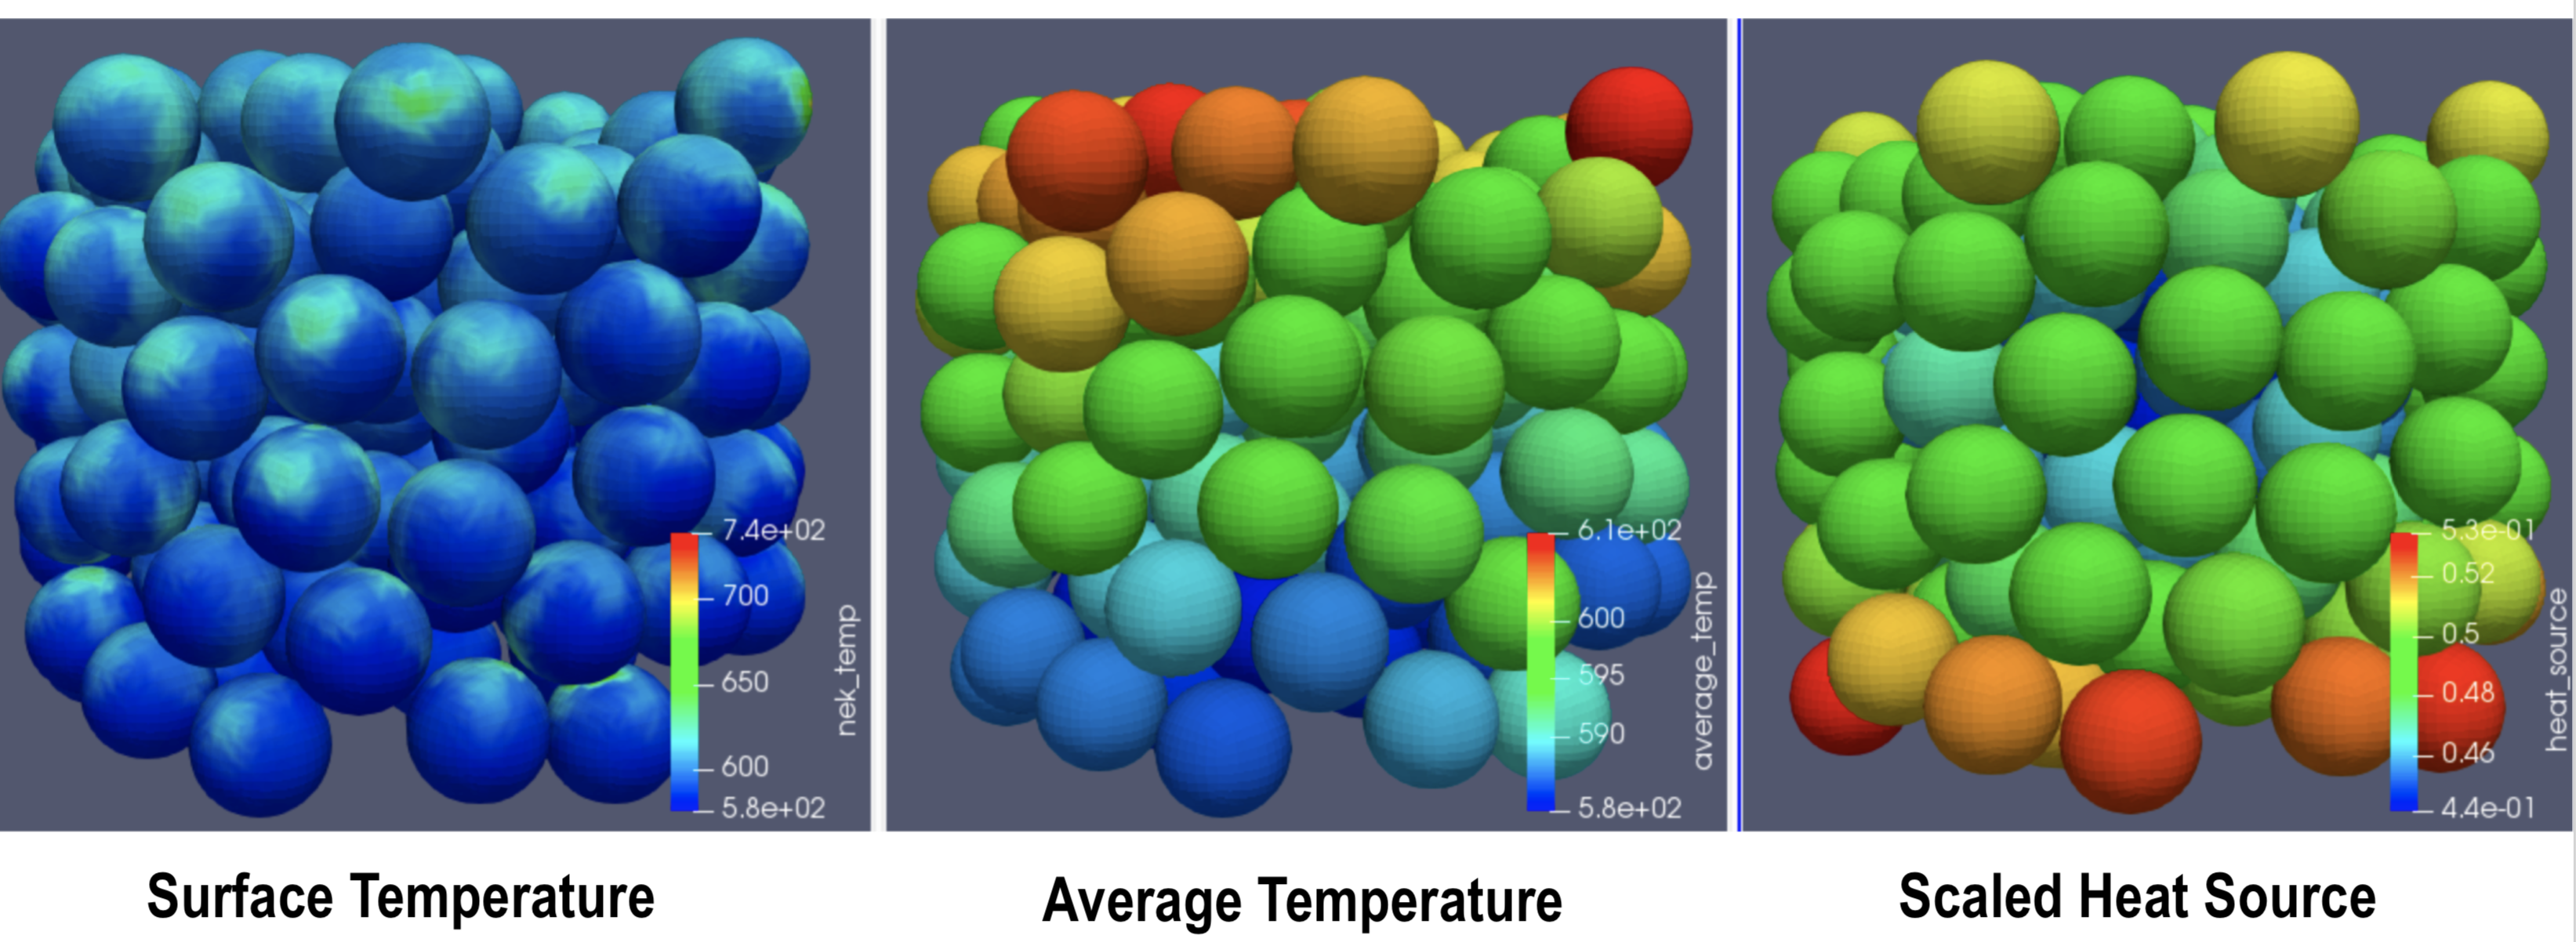
\includegraphics[clip=true,width=0.9\textwidth]{Figures/demo_r1}
\caption{TAMU demo Results. From left to right: snapshots of temperature on surface, average temperature in solid and average heating}
\label{f:dtamu1}
\end{figure}

\begin{figure}[!h]
\centering
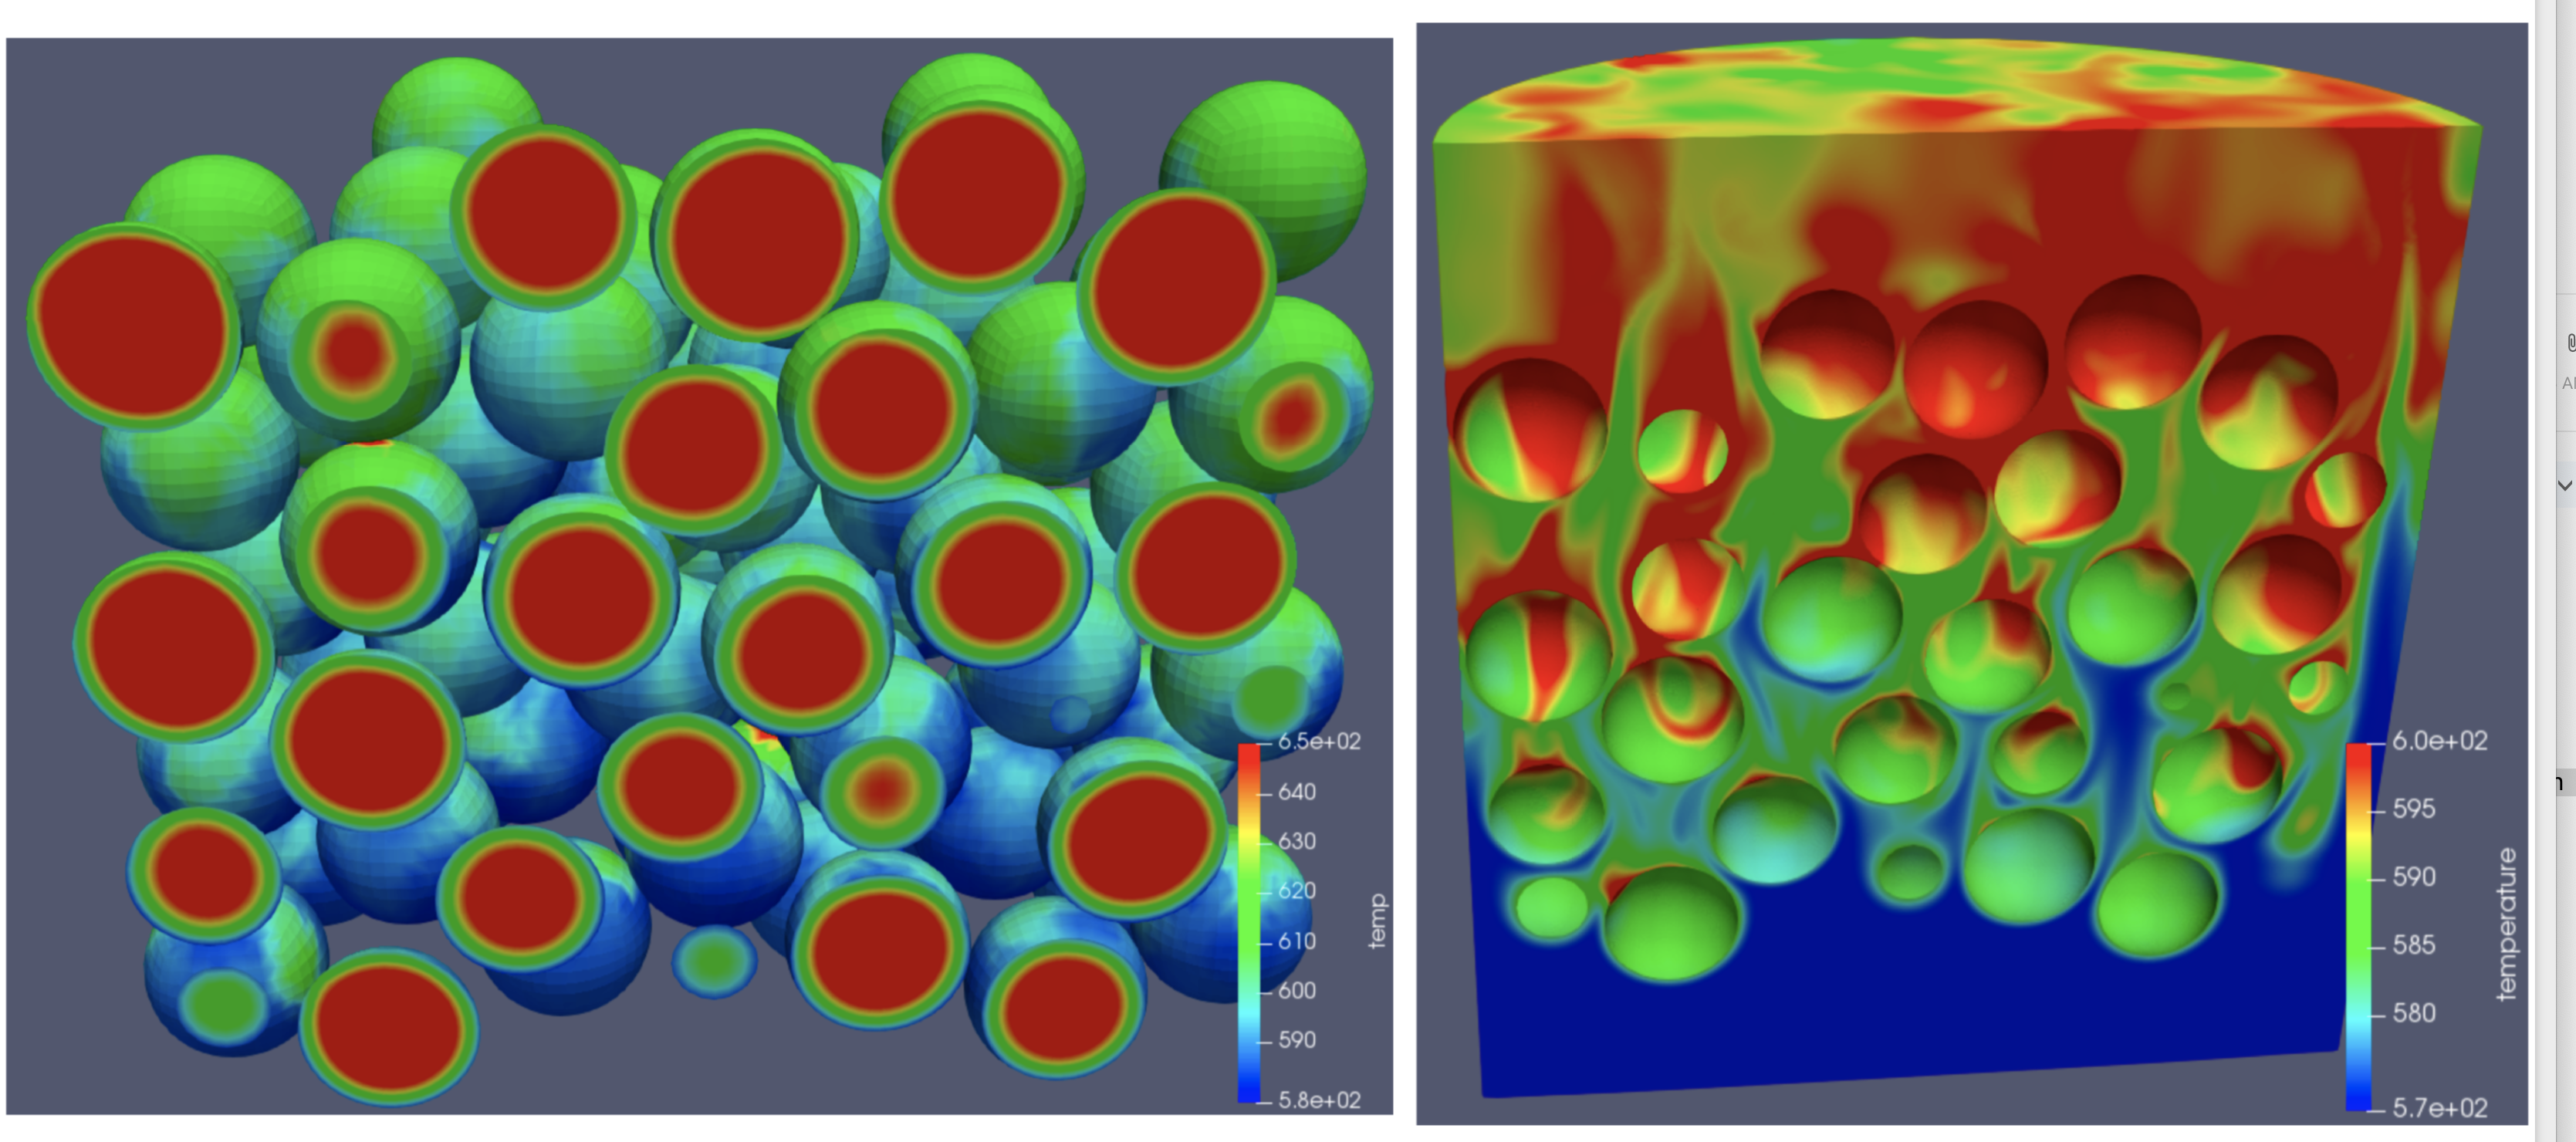
\includegraphics[clip=true,width=0.9\textwidth]{Figures/demo_r2}
\caption{TAMU Demo Results. Right - temperature in the solid. Left - temperature details in the fluid.}
\label{f:dtamu2}
\end{figure}
